% hawcx-manager — Build-Out Audit & Architecture Review
% Compile with: pdflatex HAWCX_MANAGER_AUDIT.tex  (run twice for TOC + refs)
% Requires: tikz, listings, booktabs, geometry, hyperref, xcolor, fancyhdr,
%           mdframed, enumitem, tabularx

\documentclass[11pt, a4paper]{article}

% ── Page geometry ────────────────────────────────────────────────────────────
\usepackage[
  top=2.4cm, bottom=2.4cm,
  left=2.5cm, right=2.5cm,
  headheight=14pt
]{geometry}

% ── Fonts & encoding ─────────────────────────────────────────────────────────
\usepackage[T1]{fontenc}
\usepackage[utf8]{inputenc}
\usepackage{lmodern}
\usepackage{microtype}
\usepackage{amssymb}      % \checkmark
\setlength{\headheight}{22pt}
\setlength{\emergencystretch}{2em}

% ── Colour palette ───────────────────────────────────────────────────────────
\usepackage[dvipsnames]{xcolor}
\definecolor{hawcxblue}{HTML}{1A56DB}
\definecolor{hawcxdark}{HTML}{1E3A8A}
\definecolor{hawcxgray}{HTML}{F3F4F6}
\definecolor{hawcxborder}{HTML}{D1D5DB}
\definecolor{hawcxmuted}{HTML}{6B7280}
\definecolor{accentred}{HTML}{B91C1C}
\definecolor{accentgreen}{HTML}{15803D}
\definecolor{accentamber}{HTML}{B45309}
\definecolor{accentpurple}{HTML}{6D28D9}
\definecolor{codebg}{HTML}{F8F9FA}
\definecolor{nodeblue}{HTML}{DBEAFE}
\definecolor{nodegreen}{HTML}{D1FAE5}
\definecolor{nodeamber}{HTML}{FEF3C7}
\definecolor{noderose}{HTML}{FFE4E6}
\definecolor{nodegray}{HTML}{E5E7EB}
\definecolor{nodepurple}{HTML}{EDE9FE}

% ── Tables ───────────────────────────────────────────────────────────────────
\usepackage{booktabs}
\usepackage{tabularx}
\usepackage{array}
\usepackage{caption}
\newcolumntype{L}[1]{>{\raggedright\arraybackslash}p{#1}}

% ── Lists ────────────────────────────────────────────────────────────────────
\usepackage{enumitem}
\setlist{itemsep=2pt, topsep=4pt, parsep=0pt}

% ── Code listings ────────────────────────────────────────────────────────────
\usepackage{listings}
\lstset{
  basicstyle=\ttfamily\small,
  backgroundcolor=\color{codebg},
  frame=single,
  rulecolor=\color{hawcxborder},
  framesep=4pt,
  xleftmargin=6pt,
  xrightmargin=6pt,
  breaklines=true,
  showstringspaces=false,
  keywordstyle=\color{hawcxblue}\bfseries,
  commentstyle=\color{hawcxmuted}\itshape,
  stringstyle=\color{accentgreen},
  numberstyle=\tiny\color{hawcxmuted}
}
\lstdefinelanguage{rustlite}{
  morekeywords={fn,let,match,pub,use,mod,enum,struct,impl,async,await,return,
    if,else,for,in,while,loop,break,continue,as,move,mut,ref,Self,self,
    Result,Option,Some,None,Ok,Err,true,false,unreachable,box},
  sensitive=true,
  morecomment=[l]{//},
  morestring=[b]"
}

% ── Callout boxes ────────────────────────────────────────────────────────────
\usepackage[framemethod=TikZ]{mdframed}
\newmdenv[
  linecolor=hawcxblue,
  linewidth=0.5pt,
  backgroundcolor=nodeblue!40,
  innertopmargin=6pt, innerbottommargin=6pt,
  innerleftmargin=10pt, innerrightmargin=10pt,
  roundcorner=3pt
]{infobox}
\newmdenv[
  linecolor=accentamber,
  linewidth=0.5pt,
  backgroundcolor=nodeamber!50,
  innertopmargin=6pt, innerbottommargin=6pt,
  innerleftmargin=10pt, innerrightmargin=10pt,
  roundcorner=3pt
]{warnbox}
\newmdenv[
  linecolor=accentred,
  linewidth=0.5pt,
  backgroundcolor=noderose!50,
  innertopmargin=6pt, innerbottommargin=6pt,
  innerleftmargin=10pt, innerrightmargin=10pt,
  roundcorner=3pt
]{errbox}
\newmdenv[
  linecolor=accentgreen,
  linewidth=0.5pt,
  backgroundcolor=nodegreen!50,
  innertopmargin=6pt, innerbottommargin=6pt,
  innerleftmargin=10pt, innerrightmargin=10pt,
  roundcorner=3pt
]{okbox}

% ── TikZ ─────────────────────────────────────────────────────────────────────
\usepackage{tikz}
\usetikzlibrary{
  positioning, arrows.meta, fit, calc, shapes.geometric, shapes.symbols,
  backgrounds, shadows.blur, decorations.pathreplacing, decorations.markings
}

\tikzset{
  >={Stealth[length=2.4mm, width=1.8mm]},
  every node/.style={font=\sffamily\small},
  process/.style={
    rectangle, rounded corners=2pt, draw=hawcxblue, fill=nodeblue,
    minimum width=2.5cm, minimum height=0.8cm, align=center,
    inner sep=4pt, font=\sffamily\small
  },
  daemon/.style={
    rectangle, rounded corners=2pt, draw=accentgreen, fill=nodegreen,
    minimum width=2.6cm, minimum height=0.7cm, align=center,
    inner sep=4pt, font=\sffamily\small
  },
  external/.style={
    rectangle, rounded corners=2pt, draw=accentpurple, fill=nodepurple,
    minimum width=2.8cm, minimum height=0.9cm, align=center,
    inner sep=4pt, font=\sffamily\small
  },
  storage/.style={
    cylinder, shape border rotate=90, aspect=0.25, draw=accentamber,
    fill=nodeamber, minimum height=1.1cm, minimum width=1.6cm,
    align=center, inner sep=2pt, font=\sffamily\footnotesize
  },
  symlink/.style={
    rectangle, rounded corners=1pt, draw=hawcxmuted, fill=nodegray,
    minimum width=2.6cm, minimum height=0.55cm, align=center,
    font=\sffamily\footnotesize\ttfamily, inner sep=2pt
  },
  realbin/.style={
    rectangle, rounded corners=2pt, draw=accentred, fill=noderose,
    minimum width=3.6cm, minimum height=0.7cm, align=center,
    font=\sffamily\small\bfseries, inner sep=3pt
  },
  envelope/.style={
    rectangle, draw=hawcxborder, fill=hawcxgray, rounded corners=4pt,
    inner sep=10pt
  },
  flowarrow/.style={->, hawcxdark, semithick},
  netarrow/.style={->, accentpurple, semithick, dashed},
  udsarrow/.style={->, accentgreen, semithick},
  forkarrow/.style={->, accentred, semithick},
  notelabel/.style={font=\sffamily\footnotesize\itshape, hawcxmuted}
}

% ── Headers / hyperref ───────────────────────────────────────────────────────
\usepackage{fancyhdr}
\pagestyle{fancy}
\fancyhf{}
\fancyhead[L]{\small\sffamily\color{hawcxmuted}hawcx-manager Audit}
\fancyhead[R]{\small\sffamily\color{hawcxmuted}v0.1.0-alpha.10 / 2026-05-28}
\fancyfoot[C]{\small\sffamily\color{hawcxmuted}\thepage}
\renewcommand{\headrulewidth}{0.3pt}
\renewcommand{\headrule}{\hbox to\headwidth{\color{hawcxborder}\leaders\hrule height \headrulewidth\hfill}}

\usepackage[
  colorlinks=true,
  linkcolor=hawcxblue,
  urlcolor=hawcxblue,
  citecolor=hawcxblue,
  pdftitle={hawcx-manager Build-Out Audit and Architecture Review},
  pdfauthor={Hawcx Engineering},
  pdfsubject={HAAP Multi-Call Binary},
  bookmarksnumbered=true
]{hyperref}

% ── Section styling ──────────────────────────────────────────────────────────
\usepackage{titlesec}
\titleformat{\section}
  {\normalfont\Large\bfseries\color{hawcxdark}}{\thesection}{0.6em}{}
\titleformat{\subsection}
  {\normalfont\large\bfseries\color{hawcxblue}}{\thesubsection}{0.5em}{}
\titleformat{\subsubsection}
  {\normalfont\normalsize\bfseries\color{hawcxdark}}{\thesubsubsection}{0.4em}{}

\newcommand{\code}[1]{\texttt{\small #1}}
\newcommand{\filepath}[1]{\textcolor{accentpurple}{\texttt{\small #1}}}

% =============================================================================
\begin{document}
% =============================================================================

% ── Title page ───────────────────────────────────────────────────────────────
\begin{titlepage}
\centering
\vspace*{2cm}
{\color{hawcxmuted}\sffamily\large HAAP --- Hawcx Agentic Authentication Platform}\\[0.4cm]
{\color{hawcxborder}\rule{12cm}{0.5pt}}\\[1.0cm]
{\Huge\bfseries\sffamily\color{hawcxdark} hawcx-manager}\\[0.4cm]
{\LARGE\sffamily\color{hawcxblue} Build-Out Audit \& Architecture Review}\\[1.5cm]
{\large\sffamily Multi-Call Super-Binary --- BusyBox-Style Dispatch}\\[0.3cm]
{\large\sffamily Customer-Side Runtime \& Employee-Laptop Enrollment}\\[2.0cm]

\begin{tabular}{rl}
\sffamily\color{hawcxmuted}Audit date: & \sffamily 2026-05-28\\
\sffamily\color{hawcxmuted}SDK release line: & \sffamily \code{v0.1.0-alpha.10}\\
\sffamily\color{hawcxmuted}Protocol spec: & \sffamily HAAP CS v7.2.5\\
\sffamily\color{hawcxmuted}Crate home: & \sffamily \code{hx\_agent\_client\_auth\_service}\\
\sffamily\color{hawcxmuted}Release channel: & \sffamily \code{hawcx\_agentic\_sdk}\\
\sffamily\color{hawcxmuted}Multi-call cutover: & \sffamily 2026-05-22 (Phases 1--5)\\
\end{tabular}

\vfill
{\color{hawcxborder}\rule{12cm}{0.5pt}}\\[0.3cm]
{\sffamily\footnotesize\color{hawcxmuted}
Compiled from conversational audit dated 2026-05-28.\\
Spec references: \code{HAAP-Canonical-Specification-v7\_2\_5.md},
\code{DESIGN-MEMO-MULTICALL-BINARY.md},
\code{SDK-BUILD-WITH-HAWCX-MANAGER.md}.
}
\end{titlepage}

% ── Table of contents ────────────────────────────────────────────────────────
\tableofcontents
\listoffigures
\listoftables
\clearpage

% =============================================================================
\section{Executive Summary}
% =============================================================================

\begin{okbox}
\textbf{Verdict: production-ready.} The \code{hawcx-manager} crate is structurally
complete, spec-aligned (Phases 1--5 of \code{DESIGN-MEMO-MULTICALL-BINARY.md}
landed 2026-05-22), and fully wired into the SDK release pipeline. All eight
dispatch surfaces (\code{authenticator}, \code{tqs-precompute}, \code{tqs-jit},
\code{assembler}, \code{eib}, \code{supervisor}, \code{manager}, \code{sdk})
are implemented. Build is clean (zero warnings), all 65 tests pass.
\end{okbox}

\subsection*{One-line mental model}

\code{hawcx-manager} is a BusyBox-style multi-call binary. It is one Rust ELF
that, depending on \code{argv[0]} (the symlink it was invoked through) or
\code{argv[1]} (its subcommand), behaves as one of eight roles. There is no
runtime "manager process" that "talks to" the supervisor --- \emph{the
supervisor is the same binary, invoked under a different name.}

\subsection*{Where the binary talks to the network}

Three of the eight roles open a network socket; the other five are local-only.

\begin{center}
\renewcommand{\arraystretch}{1.25}
\begin{tabularx}{\textwidth}{L{3.7cm} L{4.4cm} L{3.2cm} X}
\toprule
\textbf{Role} & \textbf{Endpoint} & \textbf{Transport} & \textbf{Purpose}\\
\midrule
\code{manager} (laptop) & CAA \code{/v1/enroll} & HTTPS + JSON & Employee enrollment\\
\code{supervisor} (container) & CAA supervisor-control & mTLS gRPC stream & Receive provisioning ops\\
\code{supervisor} (first launch) & AS \code{/v1/supervisor/bootstrap} & HTTPS + OTRC + CSR & Obtain own mTLS cert\\
\code{authenticator}, \code{tqs-*}, \code{assembler}, \code{eib} & --- & UDS only & No outbound network\\
\bottomrule
\end{tabularx}
\end{center}

\subsection*{The naming nuance that causes confusion}

The crate is named \code{hawcx-manager} but it is \emph{not} a single "manager"
program. The name \emph{manager} historically denoted the employee-laptop
enrollment CLI (\code{haap-manager}); in the 2026-05-22 cutover that program
became one subcommand of a unified super-binary --- and the super-binary
inherited the name. The container-side supervisor was absorbed into the
\emph{same} ELF. Filenames such as \code{caa\_channel.rs} in the supervisor
crate further muddy the water: that channel targets the \emph{Admin
Orchestrator}, not the CAA REST endpoint that the laptop enrollment client
talks to. \S\ref{sec:admin-plane} disentangles all three admin-side
endpoints.

\clearpage

% =============================================================================
\section{Crate Build-Out Status}\label{sec:buildout}
% =============================================================================

\subsection{Location and layout}

The crate lives at \filepath{hx\_agent\_client\_auth\_service/crates/hawcx-manager}.
It is a binary + library hybrid: \code{src/main.rs} is a 12-line entry point
that calls into the library crate \code{hawcx\_manager}.

\begin{lstlisting}[language=bash, basicstyle=\ttfamily\footnotesize]
hawcx-manager/
|-- Cargo.toml
|-- src/
|   |-- main.rs                       # 12 LOC entry: hawcx_manager::run(argv)
|   |-- lib.rs                        # 174 LOC top-level dispatch
|   |-- dispatch.rs                   # 218 LOC argv0/argv1 routing + 30 tests
|   |-- subcommands/
|   |   |-- mod.rs
|   |   |-- authenticator.rs          # thin -> haap_auth_bin::run_authenticator
|   |   |-- tqs_precompute.rs         # thin -> haap_tqs_precompute_bin::run
|   |   |-- tqs_jit.rs                # thin -> haap_tqs_jit_bin::run
|   |   |-- assembler.rs              # thin -> haap_assembler_bin::run_assembler
|   |   |-- eib.rs                    # thin -> haap_eib_bin::run_eib
|   |   |-- supervisor.rs             # thin -> haap_supervisor::run
|   |   |-- sdk/mod.rs                # 266 LOC: full ported SDK CLI
|   |   `-- manager/                  # laptop-side enrollment (full port)
|   |       |-- mod.rs
|   |       |-- caa_client.rs         # HTTPS to CAA /v1/enroll
|   |       |-- config.rs
|   |       |-- device_flow.rs        # OIDC device-code flow
|   |       |-- ipc.rs
|   |       |-- keystore.rs           # OS keychain seal/unseal
|   |       |-- state.rs              # ~/.hawcx/state.json
|   |       `-- commands/
|   |           |-- enroll.rs
|   |           |-- logout.rs
|   |           `-- status.rs
`-- tests/
    `-- smoke.rs                      # 3 integration tests (all pass)
\end{lstlisting}

\subsection{Cargo.toml summary}

One \code{[[bin]]} target (\code{hawcx-manager}) plus a library target
(\code{hawcx\_manager}). Direct dependencies on all six legacy
\code{*-bin} library crates (\code{haap-auth-bin}, \code{haap-tqs-precompute-bin},
\code{haap-tqs-jit-bin}, \code{haap-assembler-bin}, \code{haap-eib-bin}) plus
\code{haap-supervisor} (already a non-bin crate). Manager/SDK pull in
\code{haap-sdk-types}, \code{haap-sdk-sealer}, \code{haap-redis}, plus the
standard Tokio / Clap / Serde / Reqwest stack.

\subsection{Per-surface implementation status}

\begin{center}
\renewcommand{\arraystretch}{1.18}
\begin{tabularx}{\textwidth}{l l c X}
\toprule
\textbf{Surface} & \textbf{Wrapper} & \textbf{Status} & \textbf{Backing crate / module}\\
\midrule
\code{haap-authenticator} & thin & \textcolor{accentgreen}{$\checkmark$ complete} & \code{haap\_auth\_bin::run\_authenticator}\\
\code{haap-tqs-precompute} & thin & \textcolor{accentgreen}{$\checkmark$ complete} & \code{haap\_tqs\_precompute\_bin::run}\\
\code{haap-tqs-jit} & thin & \textcolor{accentgreen}{$\checkmark$ complete} & \code{haap\_tqs\_jit\_bin::run}\\
\code{haap-assembler} & thin & \textcolor{accentgreen}{$\checkmark$ complete} & \code{haap\_assembler\_bin::run\_assembler}\\
\code{haap-eib} & thin & \textcolor{accentgreen}{$\checkmark$ complete} & \code{haap\_eib\_bin::run\_eib}\\
\code{haap-supervisor} & adapter & \textcolor{accentgreen}{$\checkmark$ complete} & \code{haap\_supervisor::run} (returns \code{ExitCode})\\
\code{haap-manager} & full port & \textcolor{accentgreen}{$\checkmark$ complete} & \code{subcommands::manager} --- 3 verbs: \code{enroll}, \code{status}, \code{logout}\\
\code{haap-sdk} & full port & \textcolor{accentgreen}{$\checkmark$ complete} & \code{subcommands::sdk} --- 5 verbs: \code{run-pipeline}, \code{run-rsv}, \code{substrate-fetch}, \code{seal}, \code{unseal}\\
\bottomrule
\end{tabularx}
\captionof{table}{Per-role dispatch status. Zero \code{unimplemented!()},
\code{todo!()}, or \code{FIXME} markers anywhere in the crate.}
\end{center}

\subsection{Build, tests, and toolchain}

\begin{itemize}
  \item \code{cargo check -p hawcx-manager} --- passes in $\approx$7.8\,s,
        zero warnings.
  \item \code{cargo build --release -p hawcx-manager} --- succeeds, single
        $\approx$40\,MB binary (versus the prior $\approx$90--180\,MB
        spread across nine separate binaries).
  \item Unit tests: 62 pass --- 30 dispatch routing tests + 32 manager / SDK
        domain tests (config, keystore, IPC, device-flow, state roundtrips).
  \item Integration: \filepath{tests/smoke.rs} --- 3 pass
        (\code{--version}, \code{--help} lists all 13 subcommands,
        unknown-subcommand exits nonzero).
\end{itemize}

\subsection{Spec alignment}

Cross-checked against three canonical-spec documents:

\begin{itemize}
  \item \filepath{HAAP-TOPOLOGY-MAPPING.md} --- confirms
        \code{hx\_agent\_client\_auth\_service} owns the multi-call super-binary.
  \item \filepath{DESIGN-MEMO-MULTICALL-BINARY.md} --- Phases 1--5 landed
        2026-05-22. Phase 6 (deleting deprecated \code{[[bin]]} targets from
        the six \code{*-bin} shims) is intentionally deferred.
  \item \filepath{SDK-BUILD-WITH-HAWCX-MANAGER.md} --- Dockerfile + release
        workflow describe the symlink-fan-out post-cutover.
\end{itemize}

\subsection{Release-channel integration}

\begin{itemize}
  \item \filepath{Dockerfile} line 64 builds only the \code{hawcx-manager}
        binary target; lines 71--79 create seven symlinks
        (\code{haap-authenticator}, \code{haap-tqs-precompute},
        \code{haap-tqs-jit}, \code{haap-assembler}, \code{haap-eib},
        \code{haap-supervisor}, \code{haap-sdk}); ENTRYPOINT defaults to
        \code{haap-supervisor}.
  \item \filepath{.github/workflows/release.yml} \code{build-distribution}
        job builds the single target, packages with symlinks (Unix) or
        \code{.exe} copies (Windows), uploads as \code{docker-bins}; the
        Docker job re-creates symlinks after download.
\end{itemize}

\clearpage

% =============================================================================
\section{Architecture: Multi-Call Binary Dispatch}\label{sec:dispatch}
% =============================================================================

The crate implements the classic BusyBox pattern: a single executable
inspects \code{argv[0]} at startup, looks up a role by basename, and
branches into the role-specific entry point. Eight legacy command-line
names plus the canonical \code{hawcx-manager} name all resolve into the
same \code{.text} segment.

\subsection{Dispatch logic}

\begin{lstlisting}[language=rustlite, basicstyle=\ttfamily\footnotesize]
// crates/hawcx-manager/src/dispatch.rs
pub enum Role {
    Authenticator, TqsPrecompute, TqsJit,
    Assembler, Eib, Supervisor,
    Manager, Sdk,
    Direct,                         // unknown argv[0] -> route via argv[1]
}

pub fn role_from_argv0(argv0: Option<&str>) -> Role {
    let stem = basename(argv0).strip_suffix(".exe").unwrap_or(basename);
    match stem {
        "haap-authenticator"  => Role::Authenticator,
        "haap-tqs-precompute" => Role::TqsPrecompute,
        "haap-tqs-jit"        => Role::TqsJit,
        "haap-assembler"      => Role::Assembler,
        "haap-eib"            => Role::Eib,
        "haap-supervisor"     => Role::Supervisor,
        "haap-manager"        => Role::Manager,
        "haap-sdk"            => Role::Sdk,
        _                     => Role::Direct,
    }
}
\end{lstlisting}

When \code{argv[0]} is the canonical name (\code{hawcx-manager}) the
dispatcher falls through to \code{argv[1]} subcommand routing
(\code{enroll}, \code{status}, \code{authenticator}, \code{run-pipeline},
\dots). When \code{argv[0]} is a legacy symlink, the role is dispatched
directly with the full argv preserved so the underlying daemon sees its
conventional argv shape for logging and clap parsing.

\subsection{Figure: dispatch fan-out from a single ELF}

\begin{figure}[h]
\centering
\resizebox{\textwidth}{!}{%
\begin{tikzpicture}[
  symlinkbox/.style={
    rectangle, rounded corners=1pt, draw=hawcxmuted, fill=nodegray,
    minimum width=3.2cm, minimum height=0.6cm, align=center,
    font=\sffamily\footnotesize\ttfamily, inner sep=2pt
  }
]

% ── Section label: "on disk" ─────────────────────────────────────────────────
\node[font=\sffamily\footnotesize\itshape, hawcxmuted, anchor=west]
  at (-9.5, 8.2) {\textbf{On disk (eight filenames, one inode):}};

% ── Row 1 of symlinks (y=7.0) ────────────────────────────────────────────────
\node[symlinkbox] (s1) at (-6.6, 7.0) {haap-supervisor};
\node[symlinkbox] (s2) at (-2.2, 7.0) {haap-authenticator};
\node[symlinkbox] (s3) at ( 2.2, 7.0) {haap-tqs-precompute};
\node[symlinkbox] (s4) at ( 6.6, 7.0) {haap-tqs-jit};

% ── Row 2 of symlinks (y=5.6 — 1.4cm gap between row centers) ────────────────
\node[symlinkbox] (s5) at (-6.6, 5.6) {haap-assembler};
\node[symlinkbox] (s6) at (-2.2, 5.6) {haap-eib};
\node[symlinkbox] (s7) at ( 2.2, 5.6) {haap-manager};
\node[symlinkbox] (s8) at ( 6.6, 5.6) {haap-sdk};

% ── Convergence rail (y=4.0 — 1.3cm below row 2) ─────────────────────────────
\draw[hawcxmuted, semithick] (-7.0, 4.0) -- (7.0, 4.0);
\foreach \s in {s1,s2,s3,s4,s5,s6,s7,s8} {
  \draw[->, hawcxmuted, thin] (\s.south) -- (\s.south |- 0,4.0);
}

% ── The real binary (y=2.5) ──────────────────────────────────────────────────
\node[realbin, minimum width=5.4cm, minimum height=1.1cm] (elf) at (0, 2.5)
  {hawcx-manager\\\small\mdseries(single Rust ELF, $\approx$40\,MB)};
\draw[->, hawcxmuted, semithick] (0, 4.0) -- (elf.north)
   node[midway, right, notelabel] {symlinks resolve to one inode};

% ── "Runtime" label (y=0.9 — between ELF.south=1.95 and dispatch.north=0.4) ──
\node[font=\sffamily\footnotesize\itshape, hawcxmuted, anchor=west]
  at (-9.5, 0.9) {\textbf{At runtime (kernel exec preserves argv[0]):}};

% ── Dispatch table (y=-1.4, height 3.6cm → top=0.4, bottom=-3.2) ─────────────
\node[process, minimum width=15.0cm, minimum height=3.6cm,
      align=left, fill=nodeblue!40, inner sep=10pt] (disp) at (0, -1.4)
  {\textbf{\sffamily\small dispatch::role\_from\_argv0(basename(argv[0])) \(\longrightarrow\) Role}\\[4pt]
   \footnotesize \texttt{"haap-supervisor"      \(\to\) Role::Supervisor       (container ENTRYPOINT)}\\
   \footnotesize \texttt{"haap-authenticator"   \(\to\) Role::Authenticator    (forked by supervisor)}\\
   \footnotesize \texttt{"haap-tqs-precompute"  \(\to\) Role::TqsPrecompute    (forked by supervisor)}\\
   \footnotesize \texttt{"haap-tqs-jit"         \(\to\) Role::TqsJit           (forked by supervisor)}\\
   \footnotesize \texttt{"haap-assembler"       \(\to\) Role::Assembler        (forked by supervisor)}\\
   \footnotesize \texttt{"haap-eib"             \(\to\) Role::Eib              (forked by supervisor)}\\
   \footnotesize \texttt{"haap-manager"         \(\to\) Role::Manager          (laptop enrollment CLI)}\\
   \footnotesize \texttt{"haap-sdk"             \(\to\) Role::Sdk              (SDK demo CLI)}\\
   \footnotesize \texttt{"hawcx-manager"        \(\to\) Role::Direct \(\to\) argv[1] subcommand}};

% Arrow from ELF down to dispatch table (clear vertical run, label to right)
\draw[flowarrow] (elf.south) -- (disp.north)
   node[midway, right=4pt, notelabel] {kernel preserves argv[0]};

% ── Side annotation, parked clear of everything ──────────────────────────────
\node[font=\sffamily\footnotesize\itshape, hawcxmuted, align=left, anchor=west,
      draw=hawcxborder, rounded corners=2pt, fill=hawcxgray, inner sep=4pt]
  at (8.2, 2.5) {Unix: symlinks\\Windows: \code{.exe} copies};

\end{tikzpicture}
}
\caption{BusyBox-style multi-call fan-out. Eight symlinks (or \code{.exe}
copies on Windows) all resolve to the same \code{hawcx-manager} ELF on
disk. At runtime, the kernel preserves \code{argv[0]} across
\code{exec()}; the dispatcher branches on \code{basename(argv[0])} into
one of nine roles (eight legacy names plus the canonical
\code{hawcx-manager} which routes by \code{argv[1]}).}
\label{fig:dispatch}
\end{figure}

\clearpage

% =============================================================================
\section{Two Deployment Contexts, One Binary}\label{sec:contexts}
% =============================================================================

The same \code{hawcx-manager} ELF is deployed in two physically distinct
contexts, with completely different lifecycles:

\begin{itemize}
  \item \textbf{Customer container} (\code{ghcr.io/hawcx/hx-agent-sdk})
        --- long-running. ENTRYPOINT is the \code{haap-supervisor} symlink,
        which dispatches to \code{Role::Supervisor}; that role then forks
        five children, each of which is also \code{hawcx-manager} invoked
        under a different legacy symlink name.
  \item \textbf{Employee laptop} --- one-shot. Operator runs
        \code{hawcx-manager enroll \dots} (or the legacy \code{haap-manager}
        symlink). Talks to the CAA REST endpoint over HTTPS, seals the
        returned credentials into the OS keychain, exits.
\end{itemize}

\subsection{Figure: customer-container fork tree}

\begin{figure}[h]
\centering
\resizebox{\textwidth}{!}{%
\begin{tikzpicture}[node distance=0.7cm and 0.5cm]

% Container envelope
\begin{scope}[on background layer]
\node[envelope, minimum width=15cm, minimum height=8.5cm] (cont) at (0,-3) {};
\end{scope}
\node[anchor=north west, font=\sffamily\small\bfseries, hawcxdark]
  at (cont.north west) {\hspace{4pt}Customer container (\code{ghcr.io/hawcx/hx-agent-sdk})};

% Container ENTRYPOINT
\node[process, fill=noderose, draw=accentred] (entry) at (0, -0.5)
  {\code{ENTRYPOINT = haap-supervisor}\\
   \footnotesize(symlink $\rightarrow$ hawcx-manager)};

% Supervisor process
\node[process, fill=nodeblue, draw=hawcxblue, minimum width=4cm, below=0.8cm of entry] (sup)
  {\textbf{\code{haap-supervisor}} process\\
   \footnotesize argv[0]=\code{haap-supervisor}\\
   \footnotesize $\rightarrow$ \code{Role::Supervisor}};

% Children row
\node[daemon, below=2.6cm of sup, xshift=-5.6cm] (auth) {\code{haap-authenticator}\\\footnotesize IK\_i holder};
\node[daemon, right=0.25cm of auth] (pre)  {\code{haap-tqs-precompute}};
\node[daemon, right=0.25cm of pre]  (jit)  {\code{haap-tqs-jit}};
\node[daemon, right=0.25cm of jit]  (asm)  {\code{haap-assembler}\\\footnotesize K\_req/K\_resp};
\node[daemon, right=0.25cm of asm]  (eib)  {\code{haap-eib}\\\footnotesize \S45 OAuth};

% UDS sockets layer (conceptual)
\node[storage, below=1.4cm of pre, xshift=1.5cm, minimum width=8cm] (uds)
  {local UDS sockets\\\footnotesize framed JSON, 64\,KiB cap};

% External clients
\node[external, left=1.0cm of auth, yshift=-1.5cm] (sdk)
  {Node / Python\\SDK process\\\footnotesize (this repo)};

% Fork arrows
\foreach \c in {auth, pre, jit, asm, eib} {
  \draw[forkarrow] (sup.south) .. controls +(0,-0.3) and +(0,0.6) .. (\c.north)
       node[pos=0.55, sloped, notelabel, above=-2pt] {fork+exec};
}

% Entry to supervisor
\draw[flowarrow] (entry.south) -- (sup.north) node[midway, right, notelabel] {kernel exec};

% Children to UDS bus (one each)
\foreach \c in {auth, pre, jit, asm, eib} {
  \draw[udsarrow, <->] (\c.south) -- (\c |- uds.north);
}

% SDK to assembler
\draw[udsarrow, <->] (sdk.east) -- node[notelabel, above, sloped] {UDS} (auth.west);

\end{tikzpicture}
}
\caption{Container-side process tree. The supervisor is the only entry
point; it forks the five daemons, each of which is the \emph{same}
\code{hawcx-manager} ELF invoked under a different legacy symlink name.
All inter-daemon traffic is local UDS.}
\label{fig:container}
\end{figure}

\clearpage

\subsection{Figure: employee-laptop enrollment flow}

\begin{figure}[h]
\centering
\resizebox{\textwidth}{!}{%
\begin{tikzpicture}[node distance=1.1cm and 1.0cm]

% Laptop envelope
\begin{scope}[on background layer]
\node[envelope, minimum width=8cm, minimum height=8cm] (lap) at (-4.5,0) {};
\end{scope}
\node[anchor=north west, font=\sffamily\small\bfseries, hawcxdark]
  at (lap.north west) {\hspace{4pt}Employee laptop};

% Cloud envelope
\begin{scope}[on background layer]
\node[envelope, minimum width=5.6cm, minimum height=8cm, fill=nodepurple!30] (cloud) at (4.0,0) {};
\end{scope}
\node[anchor=north west, font=\sffamily\small\bfseries, accentpurple]
  at (cloud.north west) {\hspace{4pt}Admin plane};

% Operator invocation
\node[process, fill=nodeblue] (cli) at (-4.5, 2.6)
  {\code{\$ hawcx-manager enroll}\\
   \footnotesize\code{--tenant acme --class browser}};

% Role::Manager
\node[process, fill=nodeblue, below=0.6cm of cli, minimum width=5cm] (role)
  {\code{Role::Manager}\\
   \footnotesize\code{subcommands::manager::dispatch}};

% device_flow / caa_client / keystore stack
\node[process, fill=nodegreen, draw=accentgreen, below=0.6cm of role, minimum width=5cm] (df)
  {\code{device\_flow.rs}\\
   \footnotesize OIDC device-code $\rightarrow$ id\_token (JWT)};
\node[process, fill=nodegreen, draw=accentgreen, below=0.4cm of df, minimum width=5cm] (cc)
  {\code{caa\_client.rs}\\
   \footnotesize \code{reqwest::Client}, HTTPS, 30\,s timeout};
\node[process, fill=nodeamber, draw=accentamber, below=0.4cm of cc, minimum width=5cm] (ks)
  {\code{keystore.rs} + \code{state.rs}\\
   \footnotesize OS keychain seal + \code{\textasciitilde/.hawcx/state.json}};

% IdP and CAA
\node[external, fill=nodepurple] (idp) at (4.0, 2.5) {Customer IdP\\(OIDC)};
\node[external, fill=nodepurple, below=1.0cm of idp] (caa)
  {CAA\\\filepath{/v1/enroll}\\\footnotesize WS-5b};

% Audit / KV substrate
\node[storage, below=0.9cm of caa] (kv) {Customer Redis\\substrate};

% Edges - laptop side
\draw[flowarrow] (cli.south) -- (role.north);
\draw[flowarrow] (role.south) -- (df.north);
\draw[flowarrow] (df.south) -- (cc.north);
\draw[flowarrow] (cc.south) -- (ks.north);

% Network edges
\draw[netarrow, <->] (df.east) -- node[notelabel, above, sloped] {OIDC device-code} (idp.west);
\draw[netarrow] (cc.east) --
   node[notelabel, above, sloped] {POST id\_token + IK\_i.pub-hash}
   (caa.west);
\draw[netarrow, <-] ([yshift=-2pt] cc.east) --
   node[notelabel, below, sloped] {org\_token + nonce}
   ([yshift=-2pt] caa.west);

% CAA writes substrate
\draw[flowarrow, accentamber] (caa.south) --
   node[notelabel, right] {writes per-class registration}
   (kv.north);

\end{tikzpicture}
}
\caption{Employee-laptop enrollment. The \code{manager} role talks to the
customer IdP (OIDC device-code) and then to the CAA's \code{/v1/enroll}.
The CAA, not the laptop, writes the resulting registration into the
customer Redis substrate; the supervisor inside the container picks it
up from Redis on a later startup.}
\label{fig:laptop}
\end{figure}

\clearpage

% =============================================================================
\section{Admin-Plane Communication}\label{sec:admin-plane}
% =============================================================================

\subsection{The customer-side network boundary: CAA is the single edge}

The customer-side runtime talks to \textbf{one cloud-edge service}: the
\textbf{CAA}~--- the Client Admin Authenticator, sourced from
\filepath{hx\_agent\_\allowbreak client\_admin\_service}. The CAA exposes
\emph{two distinct surfaces} consumed by the multi-call binary --- a REST
endpoint for laptop enrollment and a gRPC supervisor-control endpoint for
the container supervisor. Anything further inside the admin plane --- the
\emph{Admin Orchestrator}, the Auth Server, audit storage --- sits
\textbf{behind} the CAA and is reached only via CAA-internal hops. The
customer-side runtime never opens a socket to those backend services
directly.

\begin{infobox}
The env var that configures the supervisor's gRPC endpoint is
\code{HAAP\_CAA\_ORCHESTRATOR\_URL} --- read it as ``the CAA's
orchestrator-facing endpoint,'' not ``the Admin Orchestrator URL.'' The
CAA is what answers that connection; it proxies operations to and from
the Admin Orchestrator internally on the admin plane. The supervisor
crate's filename \code{caa\_channel.rs} reflects this accurately --- the
peer on the wire is the CAA.
\end{infobox}

The one exception is the supervisor's first-launch OTRC bootstrap, which
talks to the Auth Server's \code{/v1/supervisor/bootstrap} endpoint
directly. The CAA does not front this call because at first launch the
supervisor does not yet possess the mTLS material the CAA gRPC surface
requires.

\begin{center}
\renewcommand{\arraystretch}{1.35}
\begin{tabularx}{\textwidth}{L{4.8cm} L{2.4cm} X}
\toprule
\textbf{Endpoint} & \textbf{Transport} & \textbf{Caller \& purpose}\\
\midrule
\textbf{CAA} \code{/v1/enroll}\newline\textcolor{hawcxmuted}{\scriptsize\sffamily WS-5b enrollment endpoint} &
  HTTPS + JSON &
  \code{Role::Manager} on employee laptop. Enroll an agent class; receive signed org\_token + registration nonce. Two auth modes: OIDC device-flow (\code{id\_token} in body) or MDM (mTLS client cert). Endpoint hosted by \filepath{hx\_agent\_client\_admin\_service}.\\
\addlinespace[2pt]
\textbf{CAA} supervisor-control (gRPC)\newline\textcolor{hawcxmuted}{\scriptsize\sffamily CAA's orchestrator-facing surface} &
  mTLS gRPC streaming &
  \code{Role::Supervisor} in container. Persistent outbound channel \emph{to the CAA} (configured by \code{HAAP\_CAA\_ORCHESTRATOR\_URL}). Sends \code{RegisterSupervisor}, opens \code{OperationStream}, receives \code{SupervisorOperation} provisioning bundles, returns \code{DeliveryResult}/\code{RevokeResult}, reports \code{SupervisorStatus} ticks. The CAA proxies these to the Admin Orchestrator internally.\\
\addlinespace[2pt]
\textbf{AS} supervisor bootstrap\newline\textcolor{hawcxmuted}{\scriptsize\sffamily \S4.6.3 -- first-launch only} &
  HTTPS + OTRC + CSR &
  \code{Role::Supervisor} on first launch only. Generates ECDSA P-256 keypair locally, POSTs \code{\{otrc, supervisor\_csr\_pem, label, org\_id\}} to AS \code{/v1/supervisor/bootstrap} \emph{directly}. Persists the returned signed cert, zeroizes the OTRC env var. Fail-closed on error.\\
\bottomrule
\end{tabularx}
\captionof{table}{Customer-side network surface. The CAA is the only
cloud edge the supervisor talks to in steady state, with the Admin
Orchestrator sitting behind it inside the admin plane. The AS bootstrap
endpoint is a one-shot exception used only when the supervisor has no
mTLS material yet.}
\end{center}

\subsection{Figure: full customer-side network topology}

\begin{figure}[h]
\centering
\resizebox{\textwidth}{!}{%
\begin{tikzpicture}[node distance=0.8cm and 0.7cm]

% ── Admin plane envelope (large, label sits ABOVE not inside) ────────────────
\begin{scope}[on background layer]
\node[envelope, fill=nodepurple!25, minimum width=18cm, minimum height=5.0cm] (admin) at (0,6.0) {};
\end{scope}
\node[anchor=south west, font=\sffamily\small\bfseries, accentpurple]
  at ([yshift=2pt] admin.north west) {Admin plane (cloud-side) --- everything behind the CAA is internal};

% ── Backend services (top row, inside admin envelope) ────────────────────────
\node[external, fill=nodepurple!55, draw=accentpurple, dashed,
      minimum width=4.0cm, minimum height=1.2cm] (orch) at (-4.5, 7.4)
  {Admin Orchestrator\\\footnotesize behind CAA};
\node[external, fill=nodepurple!55, draw=accentpurple, dashed,
      minimum width=4.0cm, minimum height=1.2cm] (audit) at (0, 7.4)
  {Audit / Redis sync\\\footnotesize behind CAA};
\node[external, fill=nodepurple, minimum width=4.0cm, minimum height=1.2cm] (as) at (4.5, 7.4)
  {\textbf{Auth Server}\\\footnotesize\code{/v1/supervisor/bootstrap}};

% ── CAA at the customer-facing edge (bottom row of admin plane) ──────────────
\node[external, fill=nodepurple, minimum width=6.0cm, minimum height=1.4cm] (caa) at (-2.0, 5.2)
  {\textbf{CAA} \footnotesize(\filepath{hx\_agent\_client\_admin\_service})\\
   \footnotesize Surfaces: \code{/v1/enroll} (REST) + supervisor-control (gRPC)};

% Internal proxy hops (CAA <-> backends, short and clean)
\draw[->, accentpurple, semithick] (caa.north -| orch.south) -- (orch.south)
   node[midway, right, notelabel] {proxy};
\draw[<->, accentpurple, semithick] (caa.north -| audit.south) -- (audit.south);

% ── Customer container (below admin plane, separated) ────────────────────────
\begin{scope}[on background layer]
\node[envelope, minimum width=10cm, minimum height=4.6cm] (cont) at (2.5, 1.0) {};
\end{scope}
\node[anchor=south west, font=\sffamily\small\bfseries, hawcxdark]
  at ([yshift=2pt] cont.north west) {Customer container};

\node[process, fill=nodeblue, minimum width=3.4cm] (sup) at (1.0, 2.2)
  {\code{haap-supervisor}\\\footnotesize (\code{Role::Supervisor})};
\node[daemon, minimum width=3.0cm] (auth) at (-0.5, 0.4) {\code{haap-authenticator}};
\node[daemon, minimum width=3.4cm] (others) at (3.0, 0.4) {\code{tqs-*, assembler, eib}};
\node[storage, minimum width=2.0cm] (redis) at (5.5, 2.2) {Redis\\substrate};

\draw[forkarrow] (sup.south) -- (auth.north) node[pos=0.45, notelabel, left=-2pt] {fork};
\draw[forkarrow] (sup.south) -- (others.north);
\draw[udsarrow, <->] (sup.east) -- (redis.west) node[midway, notelabel, above] {read};

% ── Laptop (left of container, separated) ────────────────────────────────────
\begin{scope}[on background layer]
\node[envelope, minimum width=4.6cm, minimum height=4.2cm] (lap) at (-6.6, 1.0) {};
\end{scope}
\node[anchor=south west, font=\sffamily\small\bfseries, hawcxdark]
  at ([yshift=2pt] lap.north west) {Employee laptop};

\node[process, fill=nodeblue, minimum width=4.0cm] (mgr) at (-6.6, 1.8)
  {\code{hawcx-manager enroll}\\\footnotesize (\code{Role::Manager})};
\node[storage, minimum width=3.0cm] (kc) at (-6.6, 0.2) {OS keychain\\\footnotesize sealed creds};
\draw[flowarrow] (mgr.south) -- (kc.north);

% ── Network arrows (laptop->CAA, supervisor->CAA, supervisor->AS) ───────────
\draw[netarrow] (mgr.west) -- ++(-0.8, 0) |- (caa.west)
   node[pos=0.75, notelabel, above] {HTTPS \code{/v1/enroll}};

\draw[netarrow, <->] (sup.north) -- (sup.north |- caa.south)
   node[midway, notelabel, right=2pt] {mTLS gRPC stream};

\draw[netarrow] (sup.north east) .. controls +(2.0, 1.2) and +(-0.6, -1.8) .. (as.south)
   node[pos=0.55, notelabel, sloped, above] {first-launch OTRC + CSR};

\end{tikzpicture}
}
\caption{End-to-end customer-side network topology --- \textbf{corrected}.
The CAA is the single cloud edge the customer-side runtime talks to in
steady state. Both the laptop enrollment client and the container
supervisor open sockets \emph{to the CAA}; the Admin Orchestrator and
other admin-plane backends sit \emph{behind} the CAA and are reached only
via CAA-internal proxying. The only direct call past the CAA is the
supervisor's first-launch OTRC bootstrap to the Auth Server, which
exists precisely because the supervisor has no mTLS material yet for the
CAA gRPC surface. Solid green arrows are local UDS; dashed purple arrows
are network traffic.}
\label{fig:network}
\end{figure}

\clearpage

\subsection{Supervisor mTLS bootstrap states}

The supervisor classifies its startup environment into one of four
decisions (\filepath{caa\_bootstrap.rs:88}):

\begin{itemize}
  \item \textbf{\code{Disabled}} --- \code{HAAP\_CAA\_ORCHESTRATOR\_URL}
        unset. Legacy / standalone deployment; no admin channel.
  \item \textbf{\code{Enabled}} --- URL set, cert + key files present.
        Normal happy path: open the gRPC channel and proceed.
  \item \textbf{\code{Degraded}} --- URL set, material missing, but
        \code{HAAP\_CAA\_ALLOW\_DEGRADED=true} is set. Explicit operator
        opt-in to legacy mode despite the URL being configured.
  \item \textbf{\code{BootstrappingViaOtrc}} (WS-3) --- URL set, material
        missing, but \code{HAAP\_SUPERVISOR\_BOOTSTRAP\_OTRC} and
        \code{HAAP\_AS\_BOOTSTRAP\_URL} are present. Generates ECDSA P-256
        keypair locally, builds CSR, POSTs to the AS bootstrap endpoint,
        persists the returned cert, \emph{zeroizes the OTRC env var so a
        restart cannot replay the consumed code}. \textbf{Fail-closed} on
        any error --- a half-bootstrapped supervisor sitting in degraded
        mode while an attacker re-uses the leaked OTRC would be worse
        than refusing to start.
\end{itemize}

\subsection{Figure: supervisor bootstrap decision tree}

\begin{figure}[h]
\centering
\resizebox{\textwidth}{!}{%
\begin{tikzpicture}[node distance=0.8cm and 0.8cm,
  decision/.style={diamond, aspect=2.0, draw=hawcxblue, fill=nodeblue,
                   align=center, inner sep=2pt, font=\sffamily\footnotesize},
  state/.style={rectangle, rounded corners=2pt, draw=accentgreen,
                fill=nodegreen, align=center, font=\sffamily\footnotesize,
                inner sep=4pt, minimum width=2.6cm}
]
\node[decision] (d1) {URL set?};
\node[state, below left=1.0cm and 1.5cm of d1, fill=nodegray, draw=hawcxmuted]
   (disabled) {\code{Disabled}\\\footnotesize standalone};

\node[decision, below right=1.0cm and 1.2cm of d1] (d2) {Cert + key\\on disk?};

\node[state, right=1.5cm of d2] (enabled) {\code{Enabled}\\\footnotesize gRPC channel up};

\node[decision, below=1.0cm of d2] (d3) {OTRC + AS URL\\both set?};

\node[state, below right=0.8cm and 0.3cm of d3, fill=nodepurple, draw=accentpurple]
   (otrc) {\code{BootstrappingViaOtrc}\\\footnotesize CSR $\rightarrow$ AS, persist cert};

\node[decision, below left=0.8cm and 0.1cm of d3] (d4) {\code{ALLOW\_DEGRADED}\\\code{=true}?};
\node[state, below left=0.5cm and 0.5cm of d4, fill=nodeamber, draw=accentamber]
   (degraded) {\code{Degraded}\\\footnotesize opt-in legacy};
\node[state, below right=0.5cm and 0.0cm of d4, fill=noderose, draw=accentred]
   (fail) {Fail-closed\\\footnotesize refuse to start};

\draw[flowarrow] (d1) -- node[notelabel, sloped, above] {no} (disabled);
\draw[flowarrow] (d1) -- node[notelabel, sloped, above] {yes} (d2);
\draw[flowarrow] (d2) -- node[notelabel, above] {yes} (enabled);
\draw[flowarrow] (d2) -- node[notelabel, sloped, above] {no} (d3);
\draw[flowarrow] (d3) -- node[notelabel, sloped, above] {yes} (otrc);
\draw[flowarrow] (d3) -- node[notelabel, sloped, above] {no} (d4);
\draw[flowarrow] (d4) -- node[notelabel, sloped, above] {yes} (degraded);
\draw[flowarrow] (d4) -- node[notelabel, sloped, above] {no} (fail);
\end{tikzpicture}
}
\caption{Supervisor mTLS bootstrap classifier. Four terminal states; the
WS-3 OTRC path is the only mode that performs a CSR exchange with the
Auth Server.}
\label{fig:bootstrap}
\end{figure}

\clearpage

% =============================================================================
\section{Registration Flow: \S4.6.3}\label{sec:registration}
% =============================================================================

The §4.6.3 registration flow is where the user's earlier question pointed:
\emph{how does the authenticator's IK\_i public key end up referenced in
the signed org\_token, and what role does the supervisor play?}

\subsection{Key invariant}

\begin{infobox}
The supervisor is a \emph{pass-through with capacity / lifecycle
accounting} --- not a cryptographic participant. \code{caa\_relay.rs}
states this explicitly: \emph{``The supervisor is a pass-through; it
does not inspect or modify the cryptographic content.''} IK\_i is
generated inside the authenticator during the prepare-handshake; the
supervisor only routes the provisioning bundle (received \emph{from
the CAA}, originally minted by the Admin Orchestrator that sits behind
the CAA) down to the authenticator over UDS.
\end{infobox}

\subsection{Who does what}

\begin{itemize}
  \item \textbf{Authenticator} (during prepare-handshake) --- mints
        IK\_i + IK\_i.pub locally, persists it under a slot keyed by
        \code{prepared\_agent\_id}.
  \item \textbf{Upstream} (separate path, prepare-handshake) --- the
        IK\_i.pub hash is reported upstream during the prepare phase.
        \emph{Not} via the supervisor's gRPC relay.
  \item \textbf{Admin Orchestrator} (behind the CAA) --- signs the
        org\_token, referencing the bound IK\_i.pub hash; hands the
        bundle to the CAA, which streams it to the supervisor over the
        persistent mTLS gRPC channel. The supervisor never sees the
        Orchestrator on the wire directly.
  \item \textbf{CAA} --- the cloud edge. Terminates the supervisor's
        mTLS gRPC connection, proxies operations to and from the Admin
        Orchestrator on the admin plane, surfaces
        \code{SupervisorOperation} payloads downward to the supervisor.
  \item \textbf{Supervisor} --- receives the \code{SupervisorOperation}
        bundle from the CAA, looks up the agent's control socket via
        the canonical path convention (\code{paths::ipc\_path(\dots, "auth-control")}),
        sends \code{MSG\_REGISTER\_REQ} (0x07) over UDS carrying
        \code{\{agent\_class, subject\_user\_id, prepared\_agent\_id\}}.
        Reports \code{DeliveryResult} back to the CAA. Updates
        \code{AgentTracker} for the next \code{SupervisorStatus} tick.
  \item \textbf{Authenticator} (on \code{MSG\_REGISTER\_REQ}) --- the
        \code{prepared\_agent\_id} field tells \code{perform\_agent\_registration}
        to \emph{reuse} the IK\_i already persisted under that slot, pair
        it with the inbound signed org\_token, and complete the
        registration against the Auth Server. v7.1.1-aware authenticators
        fall through to the legacy mint-fresh path if no IK\_i is
        persisted; pre-v7.1.1 authenticators ignore the extra field.
\end{itemize}

\subsection{Figure: sequence diagram --- agent registration}

\begin{figure}[h]
\centering
\resizebox{\textwidth}{!}{%
\begin{tikzpicture}[
  >={Stealth[length=2mm, width=1.5mm]},
  msg/.style={->, semithick, hawcxdark},
  netmsg/.style={->, semithick, accentpurple, dashed},
  udsmsg/.style={->, semithick, accentgreen},
  loc/.style={font=\sffamily\footnotesize\bfseries, align=center, draw=hawcxborder, fill=hawcxgray, rounded corners=2pt, inner sep=3pt},
  lifeline/.style={hawcxborder, very thin, dashed},
  every node/.style={font=\sffamily\footnotesize}
]

% Lifelines (x-coords) -- CAA inserted between Orchestrator and Supervisor
\def\xprep{0}     % prepare-handshake (upstream)
\def\xorch{2.6}   % admin orchestrator (behind CAA)
\def\xcaa{5.6}    % CAA edge
\def\xsup{8.6}    % supervisor
\def\xauth{11.4}  % authenticator
\def\xas{14.2}    % auth server

\node[loc] (Lprep) at (\xprep, 0)  {Prepare-handshake\\\footnotesize\mdseries(upstream)};
\node[loc, fill=nodepurple!40] (Lorch) at (\xorch, 0) {Admin\\Orchestrator\\\footnotesize\mdseries(behind CAA)};
\node[loc, fill=nodepurple] (Lcaa)  at (\xcaa, 0)  {\textbf{CAA}\\\footnotesize\mdseries(cloud edge)};
\node[loc] (Lsup)  at (\xsup, 0)  {haap-\\supervisor};
\node[loc] (Lauth) at (\xauth, 0) {haap-\\authenticator};
\node[loc] (Las)   at (\xas, 0)   {Auth Server};

% Lifelines
\foreach \x in {\xprep, \xorch, \xcaa, \xsup, \xauth, \xas} {
  \draw[lifeline] (\x, -0.4) -- (\x, -9.4);
}

% Visual: CAA-internal boundary shading (between orch and CAA lifelines)
\begin{scope}[on background layer]
\fill[nodepurple!18, rounded corners=2pt] (\xorch-0.6, -0.4) rectangle (\xcaa+0.6, -9.4);
\node[anchor=south, font=\sffamily\footnotesize\itshape, accentpurple]
  at ({(\xorch+\xcaa)/2}, -9.4) {admin-plane internal hops};
\end{scope}

% Step 1: Authenticator generates IK_i
\node[draw=accentgreen, fill=nodegreen, rounded corners=2pt, inner sep=3pt]
   at (\xauth, -0.9) {\footnotesize generate IK\_i, IK\_i.pub locally};

% Step 2: report IK_i.pub-hash to prepare-handshake
\draw[netmsg] (\xauth, -1.7) -- (\xprep, -1.7)
  node[midway, above, font=\sffamily\footnotesize] {report SHA-256(IK\_i.pub), agent\_id slot};

% Step 3: prepare -> orchestrator (internal admin-plane hop)
\draw[msg] (\xprep, -2.5) -- (\xorch, -2.5)
  node[midway, above, font=\sffamily\footnotesize] {bind agent\_id $\leftrightarrow$ IK\_i.pub-hash};

% Step 4: orchestrator signs org_token
\node[draw=accentpurple, fill=nodepurple, rounded corners=2pt, inner sep=3pt]
   at (\xorch, -3.3) {\footnotesize sign org\_token \{agent\_class, subject, IK\_i.pub-hash\}};

% Step 5a: Orchestrator -> CAA (internal proxy)
\draw[msg, accentpurple] (\xorch, -4.1) -- (\xcaa, -4.1)
  node[midway, above, font=\sffamily\footnotesize] {internal proxy};

% Step 5b: CAA -> supervisor (gRPC SupervisorOperation over the wire)
\draw[netmsg] (\xcaa, -4.9) -- (\xsup, -4.9)
  node[midway, above, font=\sffamily\footnotesize] {SupervisorOperation\{ bundle \}};
\node at ({(\xcaa+\xsup)/2}, -5.25) {\footnotesize\itshape mTLS gRPC stream (customer$\to$CAA)};

% Step 6: supervisor relay to authenticator
\draw[udsmsg] (\xsup, -5.8) -- (\xauth, -5.8)
  node[midway, above, font=\sffamily\footnotesize] {MSG\_REGISTER\_REQ (0x07)};
\node at ({(\xsup+\xauth)/2}, -6.15) {\footnotesize\itshape UDS, prepared\_agent\_id};

% Step 7: authenticator pairs IK_i with signed org_token, registers
\node[draw=accentgreen, fill=nodegreen, rounded corners=2pt, inner sep=3pt, align=center]
   at (\xauth, -6.8) {\footnotesize pair signed org\_token\\with persisted IK\_i};

\draw[netmsg] (\xauth, -7.6) -- (\xas, -7.6)
  node[midway, above, font=\sffamily\footnotesize] {register: IK\_i.pub + signed org\_token};

\draw[netmsg] (\xas, -8.2) -- (\xauth, -8.2)
  node[midway, above, font=\sffamily\footnotesize] {200 OK};

% Step 8: authenticator -> supervisor success
\draw[udsmsg] (\xauth, -8.85) -- (\xsup, -8.85)
  node[midway, above, font=\sffamily\footnotesize] {register\_response OK};

% Step 9a: supervisor -> CAA DeliveryResult (over the wire)
\draw[netmsg] (\xsup, -9.15) -- (\xcaa, -9.15)
  node[midway, above, font=\sffamily\footnotesize] {DeliveryResult\{ok\}};
% Step 9b: CAA -> orchestrator (internal admin-plane hop)
\draw[msg, accentpurple] (\xcaa, -9.35) -- (\xorch, -9.35)
  node[midway, above, font=\sffamily\footnotesize] {internal hop};

\end{tikzpicture}
}
\caption{Sequence diagram for §4.6.3 agent registration --- \textbf{corrected}.
The supervisor's wire peer is the \textbf{CAA}, not the Admin Orchestrator
directly. The Orchestrator signs the org\_token inside the admin plane;
the CAA proxies the provisioning bundle outward to the supervisor over
mTLS gRPC, and proxies the supervisor's \code{DeliveryResult} back
inward. Solid green arrows are local UDS; dashed purple arrows cross the
customer$\leftrightarrow$CAA wire; solid purple arrows are admin-plane
internal hops the customer-side runtime never sees.}
\label{fig:sequence}
\end{figure}

\clearpage

% =============================================================================
\section{What Was Wrong in the First Two Passes}
% =============================================================================

\begin{warnbox}
\textbf{First-pass error.} The initial audit response asserted that
\emph{``the container-side daemons never reach out to the CAA.''} That
was wrong. The \code{haap-supervisor} role maintains a persistent
outbound \emph{mTLS gRPC stream to the CAA}, and (under the WS-3
first-launch path) also POSTs a CSR directly to the Auth Server. Four
supervisor files (\code{caa\_bootstrap.rs}, \code{caa\_channel.rs},
\code{caa\_relay.rs}, \code{otrc\_bootstrap\_client.rs} --- 1,726 LOC)
implement this and were missed in the original sweep.
\end{warnbox}

\begin{warnbox}
\textbf{Second-pass error.} The corrected first response then described
the supervisor's gRPC peer as the \emph{Admin Orchestrator} (and proposed
renaming the \code{caa\_*} files to \code{orchestrator\_*}). That was
also wrong, in the opposite direction. The supervisor's wire peer is
the \textbf{CAA}, which proxies operations to/from the Admin Orchestrator
\emph{internally on the admin plane}. The customer-side runtime never
opens a socket to the Orchestrator directly. The env var name
\code{HAAP\_CAA\_ORCHESTRATOR\_URL} encodes this precisely: the CAA's
orchestrator-facing endpoint, not the Orchestrator's own endpoint. The
filename \code{caa\_channel.rs} is accurate as written; the proposed
rename would have been a regression.
\end{warnbox}

\subsection{Source of the errors}

\begin{itemize}
  \item \textbf{First-pass:} the initial grep covered the \code{manager}
        subtree only, scoped by the laptop-enrollment framing of the
        question. Skipping \code{haap-supervisor/} omitted the entire
        1,700-LOC outbound-network block.
  \item \textbf{Second-pass:} after finding \code{caa\_channel.rs} I
        latched onto the in-file comment \emph{``supervisor connects
        outbound to Admin Orchestrator''} as authoritative. That
        in-source phrasing is a shorthand for the upstream destination
        of the operation, not the wire peer; reading just the channel
        comment without tracing the actual TLS hop and env var produced
        the wrong topology. The CAA terminates the connection; the
        Admin Orchestrator is the logical origin of the operations the
        CAA forwards.
  \item \textbf{Methodology fix:} when reasoning about cloud-edge
        topology, anchor on the env var that supplies the URL and the
        TLS peer cert, not on the in-source narrative comment. Both
        artifacts here named the CAA correctly; the prose summary
        misled.
\end{itemize}

% =============================================================================
\section{Bottom Line}
% =============================================================================

\begin{okbox}
\textbf{\code{hawcx-manager} is production-ready as a multi-call
super-binary.} All eight dispatch surfaces are wired, builds cleanly,
65/65 tests pass, fully integrated into the SDK Docker image and
release workflow. Spec Phases 1--5 of the multi-call cutover landed
2026-05-22; Phase 6 (deleting deprecated \code{[[bin]]} targets from the
six legacy \code{*-bin} shims) is intentionally deferred.
\end{okbox}

\subsection{Network surface, restated}

Three of the eight roles touch the network --- and the customer-side
runtime touches only \textbf{two cloud-edge services}: the CAA in
steady state, and (one-shot) the Auth Server for first-launch bootstrap:

\begin{enumerate}
  \item \code{Role::Manager} (laptop) $\rightarrow$ \textbf{CAA}
        \code{/v1/enroll} --- one-shot HTTPS per enrollment.
  \item \code{Role::Supervisor} (container) $\rightarrow$ \textbf{CAA}
        supervisor-control --- persistent mTLS gRPC stream,
        \code{RegisterSupervisor} + \code{OperationStream} +
        \code{ReportSupervisorStatus}. CAA proxies these to the Admin
        Orchestrator behind it on the admin plane.
  \item \code{Role::Supervisor} (container, first launch only) $\rightarrow$
        \textbf{AS} \code{/v1/supervisor/bootstrap} --- OTRC + CSR
        exchange to provision the supervisor's own mTLS material.
        Direct to AS because the supervisor has no mTLS cert yet for
        the CAA gRPC surface. Fail-closed on error.
\end{enumerate}

\subsection{Top items to monitor post-launch}

\begin{itemize}
  \item \textbf{Phase 6 cleanup:} remove the \code{[[bin]]} targets from
        the six deprecated \code{*-bin} shim crates once external
        invocations are confirmed migrated to the multi-call binary.
  \item \textbf{Per-role memory footprint:} a single fat binary means each
        forked role loads all dependencies in its address space; fine on
        current targets but worth a baseline RSS measurement at GA.
  \item \textbf{Audit logging coverage:} confirm that the supervisor's
        \code{DeliveryResult} reports flowing through the CAA contain
        enough detail for the Admin Orchestrator to reconstruct §4.6.3
        audit trails without round-tripping the customer Redis substrate.
  \item \textbf{Documentation clarity (not code):} the in-source comments
        in \code{caa\_channel.rs} should be tightened to explicitly state
        that the wire peer is the CAA and that the Admin Orchestrator is
        the upstream logical origin (only) of the operations the CAA
        proxies. The filenames themselves are correct.
\end{itemize}

\vfill
\begin{center}
{\color{hawcxborder}\rule{12cm}{0.4pt}}\\[0.2cm]
\sffamily\footnotesize\color{hawcxmuted}
End of report --- hawcx-manager Build-Out Audit, 2026-05-28.\\
Compiled from in-session investigation against
\filepath{hx\_agent\_client\_auth\_service/crates/hawcx-manager} and
\filepath{hx\_agent\_client\_auth\_service/crates/haap-supervisor}.
\end{center}

\end{document}
